\title{ICTh Formelsammlung}
\author{demianthoma}
\date{Januar 2017}

\documentclass[a4paper,10pt]{scrartcl}
\usepackage{multicol}
\usepackage{calc}
\usepackage{ifthen}
\usepackage[landscape]{geometry}
\usepackage{hyperref}
\usepackage{graphicx}
\usepackage{mathtools}
\usepackage{gensymb}
\usepackage[T1]{fontenc}
\usepackage[utf8]{inputenc}
\usepackage{amsbsy}
\usepackage{amsfonts}
\usepackage{varwidth,pst-tree,pst-eps}
\usepackage{comment}

\graphicspath{ {images/} }


% This sets page margins to .5 inch if using letter paper, and to 1cm
% if using A4 paper. (This probably isn't strictly necessary.)
% If using another size paper, use default 1cm margins.
\geometry{top=0.5cm,left=0.5cm,right=0.5cm,bottom=0.5cm}

% Turn off header and footer
\pagestyle{empty}
 

% Redefine section commands to use less space
\makeatletter
\renewcommand{\section}{\@startsection{section}{1}{0mm}%
    {-1ex plus -.5ex minus -.2ex}%
    {0.5ex plus .2ex}%x
    {\normalfont\large\bfseries}}
    
\renewcommand{\subsection}{\@startsection{subsection}{2}{0mm}%
    {-1explus -.5ex minus -.2ex}%
    {0.5ex plus .2ex}%
    {\normalfont\normalsize\bfseries}}
    
\renewcommand{\subsubsection}{\@startsection{subsubsection}{3}{0mm}%
    {-1ex plus -.5ex minus -.2ex}%
    {1ex plus .2ex}%
    {\normalfont\small\bfseries}}
    
\makeatother

% Define BibTeX command
\def\BibTeX{{\rm B\kern-.05em{\sc i\kern-.025em b}\kern-.08em
    T\kern-.1667em\lower.7ex\hbox{E}\kern-.125emX}}

% Don't print section numbers
%\setcounter{secnumdepth}{0}


\setlength{\parindent}{0pt}
\setlength{\parskip}{0pt plus 0.5ex}


% -----------------------------------------------------------------------

\begin{document}

\raggedright
\footnotesize
\begin{multicols*}{3}


% multicol parameters
% These lengths are set only within the two main columns
%\setlength{\columnseprule}{0.25pt}
\setlength{\premulticols}{1pt}
\setlength{\postmulticols}{1pt}
\setlength{\multicolsep}{1pt}
\setlength{\columnsep}{2pt}

\begin{center}
     \Large{\textbf{ICTh Formelsammlung}} \\
\end{center}

\section{Periodische Signale}
\begin{align*}
    T &= \text{Periodendauer } [s] \\
    \frac{1[s]}{T[s]} = f_0 &= \text{Grundfrequenz }[Hz]\\
    \tau &= \text{Pulsdauer }[s] \\
    \frac{\tau}{T} &=\text{duty cycle }[\%]
\end{align*}
\section{Logarithmische Skalen}
$linear$ zu $dB$:
\begin{align*}
    10*log_{10}(linear) &= dB\\
    2 &= 3dB \text{ (ca.)}\\
    10 &= 10dB\\
    100 &= 20dB\\
    1000 &= 30dB
\end{align*}

$W$att zu $dBW$att und $dbM$illiwatt

\begin{align*}
    dBW = 10 * log_{10}(Watt)\\
    dBm = dbW + 30
\end{align*}

Beispiele:

\begin{align*}
    1W &= 0dBW = 30dBm\\
    0.1W &= -10dBW = 20dBm\\
    0.01W &= -20dBW = 10dBm\\
    2W &= 3dBW = 33dBm \text{ (ca.)}
\end{align*}

$V$olt zu $dBV$olt und $dB\mu V$ (Mikrovolt)
\begin{align*}
    dBV = 20 * log_{10}(V)\\
    dB\mu V = dBV + 120
\end{align*}

Beispiele:

\begin{align*}
    1V &= 0dBV = 120db\mu V\\
    0.1V &= -20dBV = 100dB\mu V\\
    0.01V &= -40dBV = 80dB\mu V\\
    0.001V &= -60dBV = 60dB\mu V\\
    0.0001V &= -80dBV = 40dB\mu V
\end{align*}

\section{Modulationsarten}

Aplitudenmodulation: 
analog: AM, SSB, VSB
digital: FSK, MSK

Frequenzmodulation:
analog: FM
digital: FSK, MSK

Phasenmodulation:
analog: PM
digital: PSK, QPSK, DPSK, DQPSK

\subsection{Mickeymouse}
Amplitudenmodulation und Hochpassfilter, 
Fouriertransformation

\section{Abtastung}

Damit Frequenzkomponenten, die Aliasing verursachen, genügend unterdrückt werden können, muss die Grenzfrequenz fg des Tiefpassfilters ca. 10\% unter der halben Abtastfrequenz $\frac{f_s}{2}$ liegen.

\section{Ohmsches Gesetz}
$U$ = Spannung $[V]$, $I$ = Stromstärke $[A]$, $R$ = Widerstand $[\Omega]$
$$U=R*I$$

\section{Leistungen}
$P$ = Leistung in Watt $[W]$
\subsection{Momentanleistung}
$t$ = Zeit
$$p(t) = u(t) * i(t)$$
\subsection{Leistung eines Signals}
Signal $s(t)$ definiert die Spannung.
$$p(t) = \frac{s^2(t)}{R}$$

\subsection{Leistungsbedarf von Zweitoren}
Alle Verstärker, Filter usw. sind Zweitore, diese Formel muss also bei Pegelplänen meistens benutzt werden. $\hat{U}$ = Spannungsspitze am Zweitoreingang, $R$ = Zweitor Widerstand (oft $50\Omega$).

$$ P = \frac{\hat{U}^2}{2R} = \frac{(1V)^2}{2*80\Omega} = 6.25 mW $$

\section{Pegelplan}
Der Spannungsspitzenwert am Ausgang des Vorverstärkers darf $\hat{U}=1V$ an $R=80\Omega$ nicht überschreiten. Die Dämpfung des Abschwächers soll so eingestellt werden, dass der Eingangspegel am Mischer unter $+5 dBm$ bleibt.

Ablauf:

\begin{enumerate}
    \item Maximaler Pegel bestimmen
    \item Grafisch maximaler Pegel bestimmen
    \item Grafisch maximaler Pegel auf minimalen Abtragen
    \item Signaldynamik bestimmen
\end{enumerate}

$SNR_{dB} = 10*log_{10}(\frac{P_{signal}}{P_{noise}})$

\subsection{Maximaler Ausgangspegel}

$$ \tilde{P} = 10*log_{10}(\frac{P}{1mW}) = 7.96 dBm $$

\subsection{Signaldynamik}

Differenz zwischen den zwei Pegeln:

$$ S = S_{max} - S_{min} $$

\subsection{Komponenten}
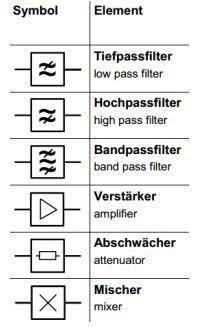
\includegraphics{komponenten}

\section{Thermische Rauschleistung}

Ein drahtloses Übertragungsystem hat eine Systembandbreite $B=160MHz$. Wie gross ist die thermische Rauschleistung [in dBm] in dieser Systembandbreite?

Formel für Raumtemperatur, Genauigkeit von $\pm$0.5db zwischen $-45\degree C$ bis $+90\degree C$.

\begin{align*}
    N &= \text{Thermische Rauschleistung} \\
    \Delta f &= \text{Systembandbreite} \\
    N &= -174dBm + 10*log_{10}(\Delta f)\\
    -174dBm + 10*log_{10}(B) &= -174dBm + 10*log_{10}(160'000'000)\\
    \text{Mit Taschenrechner}&: -174dBm + 82 = -92dBm\\
    \text{Von Hand}&: -174dBm + 10*log_{10}(2*2*2*2*10^7)\\
    -174dBm + 3dB &+ 3dB + 3dB + 3 dB + 70dB = -92dBm
\end{align*}

\section{Kanalmatrix}
\begin{align*}
    P(y_k|x_k) &= \text{Wahrscheinlichkeit, dass }y_k\text{ ankommt, wenn }x_k\text{ gesendet wird.}\\
    p &= P(y_1|x_1) \\
    1-p &= P(y_0|x_1) \\
    q &= P(y_0|x_0) \\
    1-q &= P(y_1|x_0) \\
    P(Y|X) &= \begin{bmatrix}
        p & {1-p} \\
        {1-q} & q \\
    \end{bmatrix}
\end{align*}

\subsection{Rauschfrei \& verlustfrei}

Pro Zeile und Spalte nur eine 1.

$$
P(Y|X) = \begin{bmatrix}
    1 & 0  \\
    0 & 1  \\
\end{bmatrix}
$$

\subsection{Rauschbehaftet \& verlustfrei}

Die Summe jeder Zeile muss $1$ ergeben.

$$
P(Y|X) = \begin{bmatrix}
    1 & 0   & 0   \\
    0 & 0.7 & 0.3 \\
\end{bmatrix}
$$

\subsection{Vollständig gestört}

Alle Werte sind identisch. Sie Summer der Zeilen und Spalten muss 1 ergeben.

$$
P(Y|X) = \begin{bmatrix}
    0.25 & 0.25 & 0.25 & 0.25  \\
    0.25 & 0.25 & 0.25 & 0.25  \\
    0.25 & 0.25 & 0.25 & 0.25  \\
    0.25 & 0.25 & 0.25 & 0.25  \\
\end{bmatrix}
$$

\subsection{Symbole vs. Bit}

Die Symbolrate entspricht nicht immer der Bitrate. Beispiel: ADSL hat eine Symbolrate von 4kHz. Es können aber pro Symbol mehrere Bits übertragen werden. 

Beispiel für 2 Bit pro Symbol (mit Strom):
\begin{itemize}
    \item 2V: $00$
    \item 1V: $01$
    \item -1V: $10$
    \item -2V: $11$
\end{itemize}

So ist die \textit{Symbolrate} 4kHz und die \textit{Bitrate} $$2\frac{Bit}{Symbol} * 4000 Symbole = 8000 Bit$$

\section{Entropien und maximale Symbolrate}

Die \textbf{Übertragungsrate} sei 1kbit/s. Die \textbf{Auftrittswahrscheinlichkeiten} der Zeichen der Quelle seien $p(q_0)=0.3$ und $p(q_1)=0.7$

\subsection{Informationsgehalt}
Je häufiger ein Zeichen $x_k$ auftritt, desto kleiner ist der Informationsgehalt $I(x_k)$.
\begin{align*}
I(x_k) &= log_2\left(\frac{1}{p(x_k)}\right) [bit] \\
I(x_0) &= log_2\left(\frac{1}{0.3}\right) = 1.73\text{ bits}
\end{align*}

\subsection{Entropie (der Quelle)}
Wie gross ist die Entropie $H(X)$ der Quelle (= \textbf{Mittlerer Informationsgehalt})?
\begin{align*}
    H(X) &= \sum_{k=1}^N p(x_k) * I(x_k) \\
    H(X) &= \sum_{k=1}^N p(x_k) * log_2\left(\frac{1}{p(x_k)}\right)
\end{align*}
$$\Rightarrow h\_entropy(\{0.3, 0.7\}) = 0.881291$$

\subsection{Entropie des Kanals}
Wie gross ist die Entropie $H(Y)$ des Kanals?

Gegeben ist der folgende Binärkanal mit der folgenden Kanalmatrix:

$$
P(Y|X) =
\begin{bmatrix}
    a & b  \\
    c & d  \\
\end{bmatrix}
=
\begin{bmatrix}
    0.9 & 0.1  \\
    0.1 & 0.9  \\
\end{bmatrix}
$$


\begin{align*}
    P(y_1) = a * P(x_1) + c * P(x_2) = 0.9 * 0.3 &+ 0.1 * 0.7 = \underline{0.34} (Spalte 1)\\
    P(y_2) = b * P(x_1) + d * P(x_2) = 0.1 * 0.3 &+ 0.9 * 0.7 = \underline{0.66} (Spalte 2)
\end{align*}

\begin{align*}
    H(Y) &= \sum_{k=1}^N p(y_k) * I(y_k) \\
    H(Y) &= \sum_{k=1}^N p(y_k) * log_2\left(\frac{1}{p(y_k)}\right)
\end{align*}

Falls $H(Y) = H(X)$ ist der Kanal fehlerfrei.

$$\Rightarrow h\_entropy(\{0.34, 0.66\}) = 0.924819$$

\subsection{maximale Symbolrate}
Welche maximale Symbolrate kann der Kanal fehlerfrei übertragen?

$H(Y|X)$ berechnen:
\begin{align*}
H(Y|X) = \sum_{i=1}^N \sum_{k=1}^N p(x_i)*p(y_k|x_i)*ld(p(y_k|x_i))
\end{align*}
oder mit Taschenrechner:
$$\Rightarrow h\_yx\left(\{0.3, 0.7\}, \begin{bmatrix}
    0.9 & 0.1  \\
    0.1 & 0.9  \\
\end{bmatrix}\right) = 0.468996$$

Dann Transinformation berechnen:

$$T = H(Y)-H(Y|X)$$
$$\Rightarrow t\_transinfo\left(\{0.3, 0.7\}, \begin{bmatrix}
    0.9 & 0.1  \\
    0.1 & 0.9  \\
\end{bmatrix}\right) = 0.455 Bit/Zeichen$$

Das bedeutet, die maximale Symbolrate ist $1000 \frac{Zeichen}{s} = 455 \frac{Bit}{s}$

\subsection{Entscheidungsgehalt}

Der Entscheidungsgehalt $H_0$ entspricht dem Informationsgehalt der \emph{durchschnittlichen} Auftrittswahrscheinlichkeiten

\subsection{Redundanz der Quelle}

$$R_{q}=H_0-H(x)[Bit/Zeichen]$$

\subsection{Redundanz des Codes}

$$R_{c}=L-H(x)[Bit/Zeichen]$$

wobei L die mittlere Codewortlänge ist.

\subsection{Kanalmatrix ermitteln}

Gleichungssystem lösen:
\begin{align*}
    x*0.3 + (1-x) * 0.7 &= 0.34\\
    y*0.3 + (1-y) * 0.7 &= 0.66
\end{align*}

Ergibt $x=0.9$, $y=0.1$.

$$
P(Y|X) = \begin{bmatrix}
    x & x-1  \\
    y & y-1  \\
\end{bmatrix}
$$

\subsection{Maximum Likelihood Verfahren}

$$
P(Y|X) = \begin{bmatrix}
    0.2 & \boldsymbol{0.5} & 0.3 \\
    \boldsymbol{0.7} & 0.2 & 0.1 \\
    0.4 & 0   & \boldsymbol{0.6} \\
\end{bmatrix}
$$
\\
\textbf{Entscheider:}
$y_1 = x_2$, $y_2 = x_1$, $y_3 = x_3$

\subsection{Restfehlerwahrscheinlichkeit}

$P = 1 - (0.7 * 0.6 * 0.5)$

\subsubsection{Fehlerwahrscheinlichkeit}

Die Werte $x_1=500, x_2=1200, x_3=3000$ sind gegeben.

Verteilung der entsprechenden Werte ermitteln: \\
  $p(x_1,x_2,x_3) \Rightarrow prob(\{x_1,x_2,x_3\})= 0.116, 0.253, 0.632$
  
Dann
  \begin{align*}
      &\Rightarrow res\_err\_prob(\{p(x_1),p(x_2),p(x_3)\},\{y_1=x_2,y_2=x_1,y_3=x_3\}) \\
      &\Rightarrow res\_err\_prob(\{0.116,0.253,0.632\},\{0.7,0.5,0.6\}) = 0.386
  \end{align*}

\section{Hamming-Distanz}

Die Hamming-Distanz ist der minimale Abstand zwischen zwei Codewörtern. Beim Hamming-Code ist diese 3. Falls nur die CW gegeben sind ist es die kleinste Differenz zwischen zei Codeworten. Bei zweidimensionalem Parity-Bit ergibt die Hamming-Distanz die Summe der Parity-Bits im Quadrat?

\subsection{Sicher erkennbare Fehler}
$$e^* = h-1$$

\subsection{Anzahl der sicher korrigierbaren Fehler}
\textbf{h gerade}
\begin{align*}
    h &= 2e + 2\\
    e &= \frac{h-2}{2}
\end{align*}

\textbf{h ungerade}

\begin{align*}
    h &= 2e+1\\
    e &= \frac{h-1}{2}
\end{align*}

\section{Codes}
\subsection{Anzahl Kontrollstellen k}
Wenn man eine Prüfmatrix gegeben hat, sucht man wieviele Spalten der Einheitsmatrix entsprechen. Dies ist Anzahl Kontrollstellen $k$. Zum Beispiel $k=4$

Bei zyklischen Codes ist $h=k-1$?

\subsection{Anzahl Nachrichtenstellen}
Sind die restlichen Spalten der Prüfmatrix

\subsubsection{Hamming Code}

$$m=2^k-1-k=2^4-1-4=11$$

\subsubsection{Abramsen Code}

$$m=2^{k-1}-1-k$$

\subsection{Codewortlänge}

$$CW = 2^k-1 = 2^4-1 = 15$$

\subsection{Mittlere Codewortlänge}

$$L = \sum_{i=1}^{N}p(x_i)*L(x_i) $$

$$L(x_{i})$$ ist dabei abhängig von der Codierung

Bsp:
Keine spezielle Codierung -> Zeichen A, B, C, D, E:
A = 001, B = 010, C= 011, D = 100, E = 101 
Mittlere Codewortlänge wäre hierbei 3. Nun kann es aber auch sein dass es sich um eine Huffman-Codierung handelt und darum unterschiedliche Wortlängen pro Zeichen vorhanden sind.


\subsection{Anzahl möglicher Codeworte}
Die Nachrichtenstellen $m$ plus die Kontrollstellen $k$ entsprechen der Dimension des Codes (Codestellen) $n$.
$$2^n$$
\subsection{Anzahl gültiger Codeworte}
$$2^m=2^{11}=2048$$

\subsection{Dichtgepackt?}
Der Coderaum ist dichtgepackt, wenn sich alle Codewörter (gültige und ungütige) in einer Korrigierkugel befinden.
Beispiel: $e=1$, $m=10$, $k=5$ 
$$\Rightarrow dichtgepackt(1, 10, 5)$$
oder mit der folgenden Formel:
$$2^{m}*\sum_{i=0}^{e}\binom{n}{w}=2^{n}$$
Ist die \textbf{Hammingdistanz gerade (z.B. 4)}, so kann der Coderaum \textbf{nicht dichtgepackt sein!}

\section{Zyklische Codes - Kontrollstellen ermitteln}

Gegeben ist ein zyklischer Hamming-Code mit dem Generatorpolynom $g(x)=1 + x + x^3$. Ermitteln Sie alle gültigen Codeworte durch die schnelle Mehrfachaddition

Generatorpolynom ermitteln:

$g(x)$ polynomiell ordnen: $$x^3 + x + 1$$

Dann für jede Stelle 1 (vorhanden) bzw 0 (nicht vorhanden) setzen:
$$1011$$

Dann zum Codewort ermitteln: Beispiel $1111$ (Nachrichtenteil des Codeworts)

Ziel ist es, aus dem Nachrichtenteil des Codeworts dasselbe wie das Generatorpolynom zu machen. Dies erreicht man, indem man das Generatorpolynom darunter schiebt. Rechts sind dann die Kontrollstellen zu XOR-en, um den Kontrollstellenteil des Codeworts zu erhalten

\begin{tabular}{l|l|l|l|l||r|r|r}
    Generatorpolynom & 1 & 0 & 1 & 1 \\
    Nachricht & 1 & 1 & 1 & 1 \\
    \hline\hline
    &  & 1 & 0 & 1 & 1 \\
    &  &   &  & 1 & 0 & 1 & 1\\
    \hline \hline
    &  &   &  &   & 1 & 1 & 1
\end{tabular}

Das Codewort ist nun: Nachrichtenteil + Kontrollstellen
$$1111111$$

$$\Rightarrow cyclic\_enc(1111, 1011) = 1111111$$

Nun einfach noch für alle Kombinationen der 4 Bits wiederholen.

\subsection{Irreduzibel}

Kontrollstellen k: grösstes Polynom \\
Nachrichtenanzahl m: $2^k-1-k$ \\
Codewortlänge CW: $2^k-1$

\subsection{Berechnung eines CRC-Codes mit einem gegebenen Polynom}
Bsp. Gegeben: primitives Polynom: $$1 + x + x^{4}$$
Berechnung des CRC-Code bzw. Abramson-Code:
$$((1+x+x^{4})*(1+x))mod2 = 1 + x^{2} + x^{4} + x^{5}$$
Durch die Modulo-Funktion streicht sich der Term 2x raus.\\
Nun kann daraus das Generatorpolynom gebildet werden:
$$x^{5}+x^{4}+x^{2}+1 \Rightarrow 110101$$



\section{Blockcode}

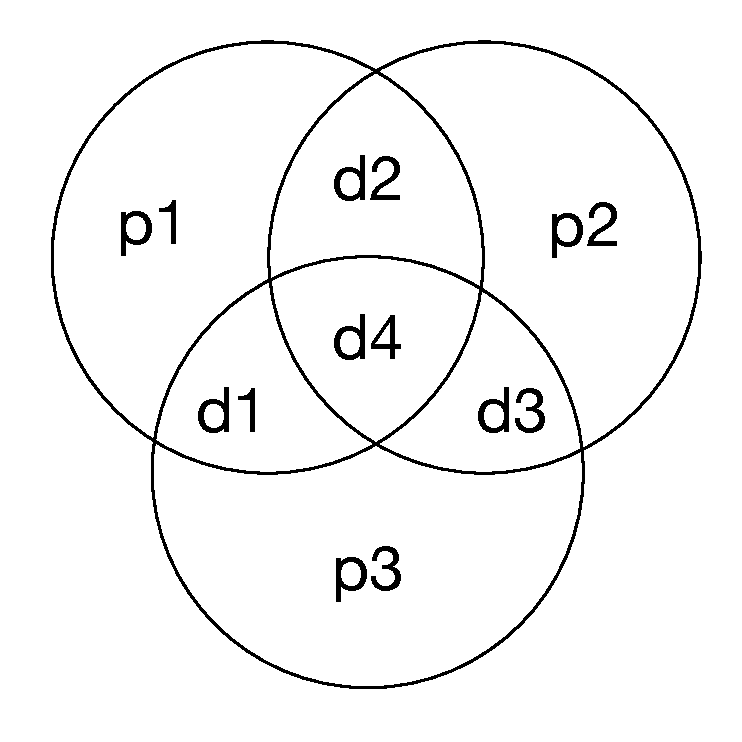
\includegraphics[scale=0.2]{hamming.pdf}

\textbf{Tailbits} entspricht der Anzahlt Speicherstellen.

\subsection{Fehlersyndrom}
Bestimmen Sie für den Fall dass $x_{12}$ und $x_{14}$ fehlerhaft sind, das Fehlersyndrom.

Lösung: Spalten quer übereinanderlegen und dann XOR-en. Falls nur 1 Spalte, = Spalte


\begin{tabular}{l|r|r|r|r}
    $x_{12}$ & 1 & 1 & 0 & 0 \\
    $x_{14}$ & 1 & 0 & 1 & 0  \\
    \hline\hline
    Fehlersyndrom & 0 & 1 & 1 & 0
\end{tabular}

Das Fehlersyndrom entspricht der Spalte des Elements, welches bei einer Vorwärtskorrektur fälschlich korrigiert würde (2 Fehlerhaft).

\subsection{Kontrollstellen ermitteln}

Gegeben: Codewort ohne Kontrollstellen, Generatormatrix

Codewort über Generatormatrix legen, alle Spalten die im Codewort $1$ sind abtragen.

\begin{tabular}{l l l|r}
1 & 1 & 0 & 0\\
1 & 0 & 1 & 0\\
1 & 1 & 1 & 1   
\end{tabular}

Kontrollstellen stehen jetzt in der rechten Spalte.



\section{Faltungscodes}

\subsection{Bedeutung der Zahlen in der Bezeichnung eines Encoders}
(Ausgang, Eingang, Speicherstellen)-Encoder\\
Bso: (2,1,3)-Encoder hat: \\
\begin{itemize}
    \item 2 Ausgänge
    \item 1 Eingang
    \item 3 Speicherstellen
\end{itemize}

$$g_1={1,1,0,1}$$
$$g_2={1,1,1,1}$$

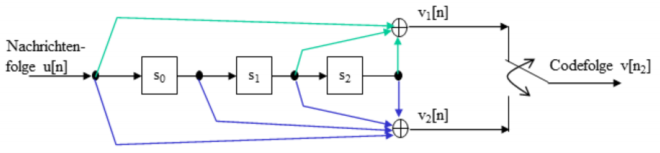
\includegraphics[scale = 0.4]{encoder}

\subsection{Zustandsautomaten für Generatorpolynom}

Gegeben: Generatorpolynome $g_1(x)=x+x^2$, $g_2(x)=1+x+x^2$

Polynome polynomiell ordnen, dann in Binär umwandeln. In unserem Beispiel:

$$\Rightarrow faltung\_dea(\{110, 111\})$$

Der TR druckt dann textweise einen Zustandsautomaten aus. Scrollen mit den Pfeilen oben und unten am Scrollbalken!

\subsubsection{Automat lesen}

Zustände: Zustände der Speicherstellen. 

Die Übergänge sind immer nach dem Schema z.B. $1/01$ beschriftet. Das bedeutet:
\begin{itemize}
    \item 1: Input $1$
    \item 01: Output $0$ und $1$
\end{itemize}

\subsection{Wieviele Zustände hat der Coder?}
$$2^{\text{Anzahl Speicherstellen}} = 2^2 = 4$$

\subsection{Blockcode-Rate}
\begin{align*}
    k &= \text{Anzahl zu codierende Bits} \\
    g &= \text{Anzahl Generatorpolynome}\\
    t &= \text{Anzahl Tailbits} \\
    \text{Blockcode-Rate} &= \frac{k}{g * (k + t)}
\end{align*}

\subsection{Ist der Code "gut"?}
Ein Faltungscode ist "gut", wenn bei allen Status beide Ausgangsübergänge maximal unterschiedlich sind: \\
\textbf{Beispiel}: $S_0 \xrightarrow[]{\text{0/00}} S_1$, $S_0 \xrightarrow[]{\text{1/11}} S_2$, beide Bits unterschiedlich \\
\textbf{Negativbeispiel}: $S_0 \xrightarrow[]{\text{0/00}} S_1$, $S_0 \xrightarrow[]{\text{1/01}} S_2$, nur ein Bit unterschiedlich \\

\section{Huffman-Code}
\begin{comment}
https://lautgesetz.com/latreex/

1
-0.575
--0.308
---0.147
----A (0.0067)
----E (0.08)
---F (0.161)
--B (0.267)
-0.425
--D (0.222)
--0.203
---0.0092
----C (0.05)
----H (0.0042)
\end{comment}

Folgend ein Huffman-Baum für folgende Häufigkeiten: 

\medskip
\textbf{A}:~$0.067$, \textbf{B}:~$0.267$, \textbf{C}:~$0.05$, \textbf{D}:~$0.222$, \textbf{E}:~$0.08$, \textbf{F}:~$0.161$, \textbf{G}:~$0.111$, \textbf{H}:~$0.042$ 
\medskip

Um den Baum zu bilden werden jeweils die beiden Knoten mit den tiefsten Wahrscheinlichkeiten verbunden.

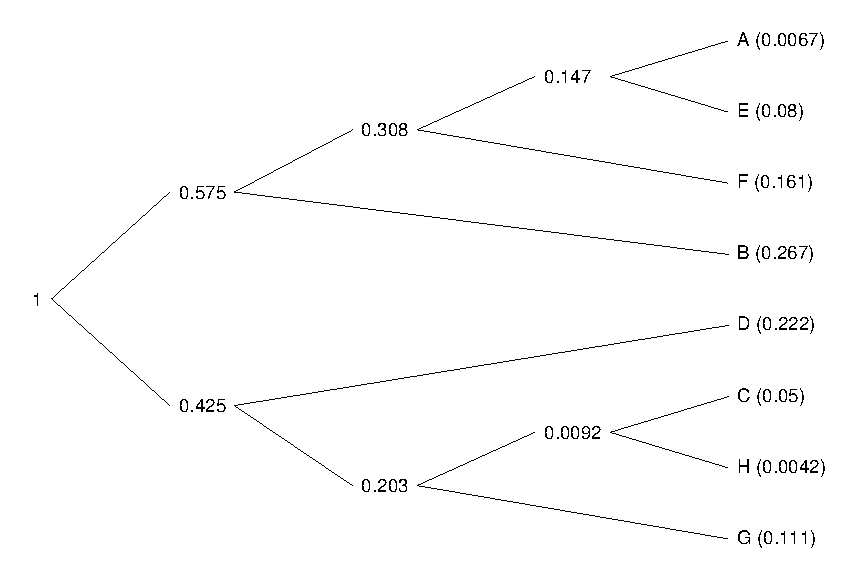
\includegraphics[scale=0.6]{huffman}

Nun entscheidet man sich einfach, ob man für oben/unten bzw. links/rechts im Baum jeweils 0 oder 1 nimmt. Dann kann man einfach ablesen. Beispiel für oben/links $0$, unten/rechts $1$:

\medskip
\textbf{A}:~$0000$, \textbf{B}:~$01$, \textbf{C}:~$1100$, \textbf{D}:~$10$, \textbf{E}:~$0001$, \textbf{F}:~$001$, \textbf{G}:~$111$, \textbf{H}:~$1101$
\medskip

\textbf{Vorteil}: Häufig vorkommende Zeichen wie B oder D brauchen nur noch 2 Zeichen, seltenere wie A brauchen 4.

\subsection{Entscheidungsgehalt}

$N$ entspricht der Anzahl verschiedener Zeichen.

$$H_0 = log_2(N)$$

\section{RSA}
\subsection{Eulerische $\varphi$() Funktion}
Gibt für jede natürliche Zahl n an, \textbf{wie viele zu n teilerfremde} natürliche Zahlen es gibt, die nicht größer als n sind:
\begin{align*}
    \varphi(n * m) &= \varphi(n) * \varphi(m)\\
    \forall p \text{ ist Primzahl} &\Leftrightarrow \varphi(p) = p - 1
\end{align*}

\subsection{Algorithmus}
\begin{enumerate}

\item Zwei Primzahlen $\boldsymbol{p}$ und $\boldsymbol{q}$ wählen. Je grösser die Primzahlen, desto sicherer.
$$p=3, q=11$$

\item Produkt $\boldsymbol{n}$ berechnen
$$n=p*q=3*11=33$$

\item $\boldsymbol{\varphi(n)}$ berechnen. Weil Faktoren von n Primzahlen sind:
$$\varphi(n) = \varphi(p*q) = \varphi(p) * \varphi(q) = (p - 1) * (q - 1) = 10 * 2 = 20$$
$$\Rightarrow rsa\_phi(33)=20$$

\item Zahl $\boldsymbol{a}$ zwischen 0 und $\varphi(n)$ finden. \textit{Bedingung}: teilerfremd zu $\varphi$(n). Idee: Primzahl nehmen, aber Teilerfremdheit prüfen.
\begin{align*}
    a &= 3\\
    0\leq a \leq \varphi(n) &\Leftrightarrow 0\leq3\leq20\\
    ggT(\varphi(n),a)&=ggT(20,3)=1
\end{align*}

\item Multiplikatives Inverses $b$, von $a$, in $\mathbb{Z}_{\varphi(n)}$ berechnen
$$a*b\equiv1\bmod \varphi(n) \Leftrightarrow 3*b\equiv1\bmod20 \Rightarrow b=7$$
$$\Rightarrow rsa\_{ereuk}(3,20) = 7.$$

\item Die Zahlen $p$, $q$ und $\varphi(n)$ werden nicht mehr benötigt.
\item \textbf{Öffentlichen Schlüssel} veröffentlichen: $n, b$
$$n=33, b=7$$

\item \textbf{Privaten Schlüssel} behalten: $n$, $a$
$$n=33, a=3$$

\item Nachricht $m$ \textbf{verschlüsseln} als $c$
$$c \equiv m^a \bmod(n)$$
$$\Rightarrow mod(m^a, n)$$

\item Nachricht $v$ zu $m$ \textbf{entschlüsseln}
$$m \equiv c^b \bmod(n)$$
$$\Rightarrow mod(c^b, n)$$
\end{enumerate}

\section{Modulationsarten}

\subsection{QPSK 2 Bit}

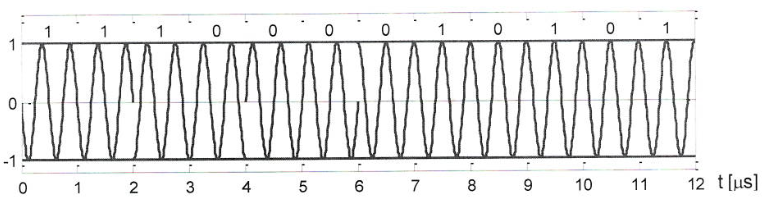
\includegraphics[scale=0.3]{qpsk.png}

\subsection{DQPSK 2 Bit}

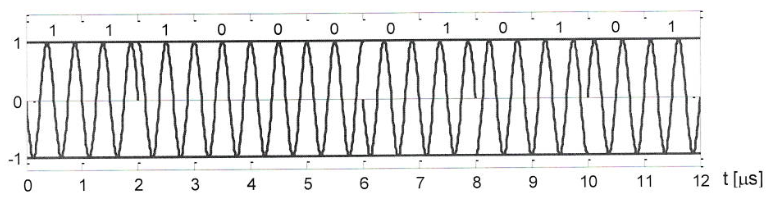
\includegraphics[scale=0.3]{dqpsk.png}

\subsection{PSK 1 Bit}

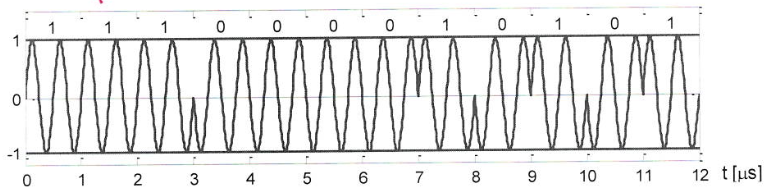
\includegraphics[scale=0.3]{psk.png}

\subsection{8-PAM / 3 Bit}

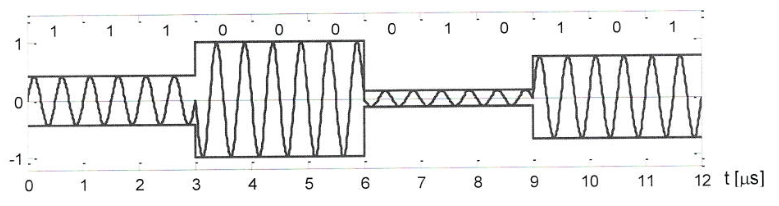
\includegraphics[scale=0.3]{8pam.png}


\end{multicols*}
\end{document}
